\documentclass[11pt,a4paper]{report}

% Packages
\usepackage[utf8]{inputenc}
\usepackage[T1]{fontenc}
\usepackage[english]{babel}
\usepackage{csquotes}
\usepackage{amsmath,amssymb,physics}
\usepackage{graphicx}
\usepackage{hyperref}
\usepackage{geometry}
\usepackage{xcolor}
\usepackage{indentfirst}
\usepackage{ragged2e}
\usepackage{tocloft}
\usepackage{lastpage}
\usepackage{fancyhdr}
\usepackage{framed}
\usepackage{stmaryrd}
\usepackage{mathtools}
\usepackage{bm}
\geometry{margin=1.5cm}

% Clean figures
\usepackage{caption}
\usepackage{subcaption}
\usepackage{chngcntr}
\counterwithout{figure}{chapter}
\counterwithout{table}{chapter}
\counterwithout{footnote}{chapter}


% Bibliography (moderne)
\usepackage[backend=biber,style=numeric,sorting=none]{biblatex}
\addbibresource{references.bib}

\begin{document}
\renewcommand{\thechapter}{\Roman{chapter}}
% \renewcommand{\thesection}{\thechapter.\roman{section}}
% \renewcommand{\thesubsection}{\Roman{chapter}.\roman{section}.\arabic{subsection}}
\renewcommand{\Tr}[1]{\operatorname{Tr}\left[#1\right]}
\renewcommand{\cfttoctitlefont}{\Huge\bfseries\MakeUppercase}
\renewcommand{\cftaftertoctitle}{
  \vskip 2.5mm
  \noindent\rule{\textwidth}{0.8pt}\\[-3 mm]
  \noindent\rule{\textwidth}{0.8pt}\\[-3 mm]
}
\pagestyle{fancy}
\fancyhf{}
\fancyfoot[C]{---\thepage/\pageref{LastPage}---}
\fancypagestyle{plain}{
  \fancyhf{}
  \fancyfoot[C]{---\thepage/\pageref{LastPage}---}
  \renewcommand{\headrulewidth}{0pt}
}


\renewcommand{\headrulewidth}{0pt}
\setlength{\cftsubsecnumwidth}{15mm}
\newcommand{\dert}[1]{\frac{\mathrm{d}#1}{\dt}}
\newcommand{\derpart}[1]{\frac{\partial#1}{\partial{}t}}
\newcommand{\nIH}{{n\in{I_\mathcal{H}}}}
\newcommand{\ito}{It\={o}}
\newcommand{\dt}{\mathrm{d}t}
\newcommand{\boldsection}[1]{\textbf{\boldmath #1}}

% ACKNOWLEDGEMENTS PAGE
\newpage\thispagestyle{empty}
\centering {\Huge \textbf{ACKNOWLEDGEMENTS}}
\vskip 2.5mm
\noindent\rule{\textwidth}{0.8pt}\\[-3    mm]
\noindent\rule{\textwidth}{0.8pt}
\vskip 5mm
\begin{justify}
    \hspace{0.5cm}The author expresses deep gratitude to Bruno Bellomo for his guidance and support throughout this research. Bruno, as a mentor, constantly took the time to explore ideas, ensure our understanding, and seek details. His expertise in Quantum Mechanics has been fundamental to the successful completion of this Master’s thesis. I am grateful to conclude my short career as a physicist with such a demanding journey, thanks to Bruno.\par\vspace{0.15cm}\noindent
    I would like to thank the members of the jury for their time and interest in this work, as well as for the opportunity to present my work in front of such esteemed peers.\par\vspace{0.15cm}\noindent
    I also would like to thank my colleagues, of a few months, for their insightful discussions and support during this internship: Silvio Da Silva, Jana El Badawi, Anjana Mohan, and Léo Jacquerot-Legros.\par\vspace{0.15cm}\noindent
    Finally, I would like to thank my friends and family for their never-ending support: Erwan Le D{\oe}uff, Titouan Alphonse, and Nabyan Arkan for these two years of Master’s studies and friendship together, also, thank to Maxence Bonin and Vincent Girod my brothers from other mothers. I owe everything to my parents, Catherine and Lionel, for my life and education, and, to my brother Pierre who is so resilient and skillful. Lastly, I want to thank my other half, Alexiane.
\end{justify}
\rule{0.5\textwidth}{1pt}\par
\vspace{0.25cm}
\begin{justify}
    \hspace{0.5cm}L'auteur exprime sa profond gratitude envers Bruno Bellomo pour ses conseils et son soutien tout au long de ce travail de recherche. Bruno, en tant que mentor, a constamment pris le temps d'explorer des idées, de s'assurer de notre compréhension et d'approfondir les détails. Son expertise en mécanique quantique a été fondamentale dans la bonne conduite de ce mémoire de master. Je suis reconnaissant de pouvoir conclure ma courte carrière de physicien par un parcours aussi exigeant, grâce à Bruno.\par\vspace{0.15cm}\noindent
    Je tiens à remercier les membres du jury pour le temps et l'intérêt qu'ils porteront à ce travail, ainsi que pour l'opportunité de le présenter devant des pairs reconnus.\par\vspace{0.15cm}\noindent
    Je souhaite tout de même remercier mes collègues de quelques mois pour leurs discussions enrichissantes et leur soutien durant ce stage: Silvio Da Silva, Jana El Badawi, Anjana Mohan et Léo Jacquerot-Legros.\par\vspace{0.15cm}\noindent
    Enfin, je tiens à remercier mes amis et ma famille pour leur soutien indéfectible~: Erwan Le D{\oe}uff, Titouan Alphonse et Nabyan Arkan pour ces deux années d'études de Master et amitié partagées, mais également, merci à Maxence Bonin et Vincent Girod mes frères d'autre mères. Je dois tout à mes parents, Catherine et Lionel, pour ma vie et mes études, ainsi qu'à mon frère Pierre qui sait être résilient et plein de ressources. Pour finir, je remercie ma meilleure moitié et compagne, Alexiane.
\end{justify}
\vfill
\begin{flushright}
    \small{\textit{« La gloire de Dieu, c'est de cacher les choses; La gloire des rois, c'est de sonder les choses. »} \\
    \textbf{— Proverbes 25:2}}
\end{flushright}\newpage

\justifying
\normalsize % SIZE OF CONTENTS!!!
\tableofcontents
\addtocontents{toc}{\protect\thispagestyle{empty}}
\clearpage

\normalsize\justifying
\setlength{\parskip}{2mm}
\setcounter{page}{1}
\section*{\Huge Introduction}
\addcontentsline{toc}{chapter}{Introduction}

``Quantum mechanics is the description of the behavior of matter and light in all details and, in particular, of the happenings on an atomic scale'' said \textit{R.Feynman} in one of his lectures~\cite{Feynman}. In this framework, position is no longer a single well-defined value prior to measurement, instead, position is described by a probability density all across space. Consequently, the notion of a trajectory as a continuous succession of points in spacetime is lost in quantum dynamics. The definition of trajectory will therefore be addressed, but one question remains paramount when mentioning systems: how can we even define a quantum system properly?\par

In the ideal case, systems are treated as \underline{closed}, i.e., isolated from any external environment and interacting with nothing at all. This modelling allows quantum mechanics to describe the dynamics of systems with unitary and deterministic terms (the state at time $t$ is determined solely by knowing the state at time $t_0$) using the Schrödinger equation.~\cite{CT}However, in the physical world, systems do ``feel'' their surroundings, \textit{i.e.}, they interact with their environment. This interaction should be taken into account to obtain a more complete and physically relevant representation. In doing so, we consider the so-called \textit{Open Quantum System} (OQS) theory~\cite{Breuer}.\par 

Other useful theories have been developed through the last decades, allowing quantum mechanics' description to be more and more complete. One of them is the Quantum Measurement Theory (QMT)~\cite{Jacobs}, where the concept of measurement is fully described. Measuring a quantum system has a tremendous impact on its properties. Furthermore, since any experimental probe inevitably interacts with the system, it is crucial to figure out the nature of this interaction. Measuring a system without impacting its properties leads to the concept of \underline{weak measurements}, that we will develop further below.\par

By studying QMT, one can thus notice that measuring a quantum system alters it. The measurement usually interacts so strongly with the system that it collapses into a state --- an eigenstate of the measured observable --- leading to a loss of the system's properties of interest. For example it can lose its entanglement\footnote{
    $\ket{\psi}_{AB}=\frac{\ket{00}+\ket{11}}{\sqrt{2}}\underset{\text{in A}}{\overset{\text{measuring 0}}{\longrightarrow}}\ket{00}_{AB}=\ket{0}_A\otimes\ket{0}_B$ a product state (thus non-entangled).
}. Along the same lines, quantum systems can be in superposition of states. To illustrate this property, we can think about the \textit{Schrödinger's cat} thought experiment, which corresponds formally to a superposition of `the cat is alive' and `the cat is dead' states prior to measurement. Measuring the state of the cat will determine its fate, alive or dead. It is then ``stuck'' in the state measured and cannot be expressed as a superposition again.
The idea of \textbf{weak measurements} is to \textbf{measure the environment} coupled with the system. Instead of altering dramatically the state of the system, we extract pieces of information about it. The measurements can even be conducted continuously, maximizing the amount of data that an observer can obtain. These are the global ideas behind \textbf{Quantum Continuous Measurements} (QCM)~\cite{Albarelli}.

Practically, this work will be organized as follows: the first chapter covers an academical progression from the basics of quantum mechanics up to the aforementioned theories. A second chapter will cover the \underline{photodetection} and \underline{homodyne detection} of the environment of open quantum systems. The final section of this second chapter presents simulation results for both the qubit and the harmonic oscillator, comparing the two detection methods on each of them.
\newpage

\chapter{Basics of quantum mechanics}\setlength{\parindent}{6mm}\setlength{\parskip}{2mm}
\section{Generalities on closed quantum systems}
\subsection{States and time evolution}\label{Ii1}\noindent
In quantum mechanics a physical system's state is described by a vector in a Hilbert space:
\begin{equation}
    \ket{\psi}\in\mathcal{H}.
\end{equation}
The Hamiltonian $\hat{H}$ is a specific Hermitian\footnote{$\hat{H}^\dagger=\hat{H}$, where $^\dagger$ denotes the conjugate transpose, defining the Hermitian adjoint. } operator representing classically the total energy of a system; this relationship will be detailed in Section~\ref{sec:obs}. Physically, the evolution of a system is governed by its energy, the \textit{Schrödinger equation} states it explicitly:
\begin{equation}
    i\hbar\frac{\mathrm{d}\ket{\psi(t)}}{\dt}=\hat{H}(t)\ket{\psi(t)}.
\end{equation}
The solution of the Schrödinger equation can be expressed as an unitary\footnote{$\hat{U}\hat{U}^\dagger=\hat{U}^\dagger \hat{U}=\mathbb{I}$, where $\mathbb{I}$ is the identity.} operator $\hat{U}$ such that,
\begin{equation}
    \ket{\psi(t)}=\hat{U}(t,t_0)\ket{\psi(t_0)},
\end{equation}
with initial condition $U(t_0,t_0)=\mathbb{I}$. By injecting the previous relation in the state equation, we get
\begin{equation}\label{eq:schrodU}
    \dert{\hat{U}}(t,t_0)=-\frac{i}{\hbar}\hat{H}(t)\hat{U}(t,t_0).
\end{equation}
We will simply assume the Hamiltonian to be time-independent in the following, nevertheless, solutions exist in the time-dependent case~\cite{Breuer}. For us, the equation of evolution, solution of the Schrödinger equation, is
\begin{equation}\label{eq:solschrod}
    \ket{\psi(t)} = \underbrace{e^{-\frac{i\hat{H}(t-t_0)}{\hbar}}}_{\hat{U}(t,t_0)}\ket{\psi(t_0)}.
\end{equation} 
This solution is indeed \textbf{unitary} and we can use $\hat{U}^\dagger(t,t_0)$ on the left of both sides of the Eq.~(\ref{eq:solschrod}) to obtain $\ket{\psi(t_0)}=\hat{U}^\dagger(t,t_0)\ket{\psi(t)}$, i.e., we described \textbf{reversible} dynamics.\newpage 
\subsection{Observables}\label{sec:obs}\noindent
In quantum mechanics, any physical quantity is represented by an \textbf{observable} which is an operator fulfilling two properties: the eigenvectors of the observable form an orthonormal basis of the Hilbert space $\mathcal{H}$, and, the corresponding eigenvalues are necessarily real~\cite{CT}. In finite-dimensional Hilbert spaces, the definition of Hermitian operator\footnote{The eigenvectors of a Hermitian operator always span the entire Hilbert space (Spectral Theorem). Using the Gram-Schmidt process, we can always find a complete orthonormal basis from the operator's eigenspaces.} is sufficient for it to be an observable. In the case of infinite dimension Hilbert spaces, the definition of an observable requires more rigorous mathematical foundations (self-adjoint operators, the details of which lie beyond the purview of this study). In this sense, we only consider finite dimension cases in the following. We thus define the interval $I_\mathcal{H}=\llbracket 1;\text{dim}(\mathcal{H})\rrbracket$ throughout this document, also, we lighten the notation by omitting $\hat{\bullet}$ symbols on operators hereafter.

 A natural operator whose eigenbasis $\qty{\ket{\phi_n}}_\nIH$ is particularly significant is the Hamiltonian $H$, as its eigenvalues $\qty{E_n}_\nIH$ correspond to the allowed energy values of a system. We can understand the relation between an operator, its eigenvectors and eigenvalues with its corresponding eigenequation:
\begin{equation}\label{eq:PropreH}
    \forall n \in I_\mathcal{H},\quad H\ket{\phi_n} = E_n\ket{\phi_n} .
\end{equation}
Since $\qty{\ket{\phi_n}}_\nIH$ forms a basis of the Hilbert space, one can describe any state $\ket{\psi}$ in this very basis:
\begin{equation}\label{eq:stateinHbasis}
    \forall\ket{\psi}\in\mathcal{H},\qquad \ket{\psi} = \sum_{n\in I_\mathcal{H}} c_n\ket{\phi_n},
\end{equation}
where $c_n=\braket{\phi_n}{\psi}$. This kind of description in a base is obviously valid for any observable, not only for the Hamiltonian. 

Finally, we mention the necessity of normalizing states, which is important when calculating probabilities (the Section~\ref{sec:qmt} makes it obvious). In order to normalize a state, one needs to set $\norm{\psi}=\sqrt{\braket{\psi}{\psi}}=1$, which is equivalent to the condition $\braket{\psi}{\psi}=\sum_n |c_n|^2=1$.

\subsection{Purity of states}\noindent
The concept of \textit{pure state} arises from the necessity to write the state of a system in a different way than that used so far in this document. Indeed, certain ways of preparing a system --- such as a statistical mixture\footnote{In the Appendix~\ref{ann:statmix}, we explain how to prepare a system as a statistical mixture or as a superposition of states. However, we recommend to read the Section~\ref{sec:qmt} on quantum measurement theory before.}--- require another formalism because such processes prevent the state of the system from being expressed as a single $\ket{\psi}$ (or as a superposition of state vectors). To take into account such cases, we introduce the density matrix hereafter.

A density matrix $\rho$ is an operator of the Hilbert space $\mathcal{H}$ (and also an operator of the dual space $\mathcal{H^*}$), which follows a set of properties:\label{prop:rho}
\begin{itemize}
    \item $\rho$ is Hermitian: $\rho=\rho^\dagger$, implying it can be diagonalized and necessarily with a positive eigenvalues, $\mathrm{Sp}(\rho)\subset\mathbb{R^+}$.
    \item $\Tr{\rho}=1$ necessarily.
    \item $\rho$ is positive semi-definite: $\forall\ket{\psi}\in\mathcal{H},\quad \expval{\rho}{\psi}\geq 0$.
\end{itemize}\newpage\noindent
The density matrix formalism is particularly useful because it generalizes Dirac formalism. Indeed, if a state can be written as $\ket{\psi}$ then $\rho=\ketbra{\psi}$ and we call it a \textbf{pure state}. Otherwise, the state is non-pure and can only be expressed with a density matrix. Also, pure states satisfy stronger properties than those defining a general density matrix; specifically, being idempotent $\rho^2=\rho$ by construction, implying that $\Tr{\rho^2}=\Tr{\rho}=1$ in the case of pure states.
\subsection{Postulates of quantum mechanics}\noindent
Physicists developed a corpus of the main properties of quantum mechanics, here are summarized the so-called postulates of quantum mechanics~\cite{CT}:
\begin{enumerate}
    \item The state of a system is represented by a density matrix $\rho\in\mathrm{End}(\mathcal{H})$ respecting properties~\ref{prop:rho}. For pure states we can describe them $\ket{\psi}\in\mathcal{H}$, or, by using the pure matrix density formalism $\rho_p=\ketbra{\psi}{\psi}$. 
    \item Physical quantities $\mathcal{A}$ are associated with operators $\hat{A}$, called observables. In the context of finite dimension space, they are simply Hermitian operators.
    \item The only possible outcomes of a measurement of $\mathcal{A}$ are the eigenvalues $a$ of $\hat{A}$, defined by $\hat{A}\ket{a}=a\ket{a}$\label{pstlt:3}.
    \item When measuring $\mathcal{A}$ on a normalized state, we know the probability to get one of the possible eigenvalues: $\mathbb{P}[a_n]$ (which depends on the spectrum of the observable).
    \item If the measurement of the physical quantity $\mathcal{A}$ on the system gives the result $a_n$, the state of the system immediately after the measurement collapses into the eigenstate $\ket{\phi_n}$.
    \item The time evolution of the wavefunction $\ket{\psi(t)}$ is governed by the \textit{Schrödinger} equation:
    \begin{equation}
    \frac{\mathrm{d}\ket{\psi(t)}}{\mathrm{d} t}=-\frac{i}{\hbar}H(t)\ket{\psi(t)}.
    \end{equation}
    For density matrices, the evolution is driven by the \textit{Liouville-von Neumann} equation:
    \begin{equation}\label{eq:Liouville}
        \frac{\mathrm{d}\rho}{\dt}(t) = -\frac{i}{\hbar}\left[ H(t),\rho(t)\right]\footnotemark[1].
    \end{equation}
\end{enumerate}
\footnotetext[1]{$[\hat{A},\hat{B}]=\hat{A}\hat{B}-\hat{B}\hat{A}$ is called the commutator of $\hat{A}$ and $\hat{B}$.}

\section{Multipartite systems}\label{sec:multipartite}
\subsection[Quantum measurement theory]{Quantum Measurement Theory (QMT)}\setlength{\parindent}{2mm}
\noindent
We recall the Postulate~\ref{pstlt:3}, defining $a$ and $\ket{a}$ from $A\ket{a}=a\ket{a}$. In the QMT~\cite{W94,W96}, measuring consists in applying a projector to a state, thus we call this process a \textit{projective measurement}. The set of projective measurements is called a Projection-Valued Measure (PVM)~\cite{Holevo}. Since an observable has a set of eigenvectors, we can build a projector corresponding to one of them:
\begin{equation}
    P_a = \ketbra{a}.
\end{equation}
This definition implies four important properties: 
\begin{equation*}
    P_a^\dagger = P_a, \qquad
    P_a^2 = P_a, \qquad
    P_a P_b = P_a \delta_{ab}, \qquad
    \sum_n P_{a_n}=\mathbb{I}.
\end{equation*}
In the last property, $n$ is an index representing one measurement result among every possible result. For an observable with a non-degenerate spectrum, the set of measurement results is indexed by $I_\mathcal{H} = \llbracket 1, \dim(\mathcal{H}) \rrbracket$. The probability to measure $a$ is defined by
\begin{align}
    \mathbb{P}_{\ket{\psi}}[a] &= \expval{P_a}{\psi}\\
    &= \abs{\braket{\psi}{a}}^2,\\
    \mathbb{P}_{\rho}[a] &= \Tr{\rho P_{a}}.
\end{align}
The theory stipulates that states collapse after measurement. The unnormalized state (denoted by $\tilde{}\;$) is thus
\begin{align}
    \tilde{\ket{\psi_a}} &= P_a\ket{\psi},\\
    \tilde{\rho_a} &= P_a\rho P_a.
\end{align}
The obtained state is said \textbf{conditioned by the measurement} result $a$, hence the importance of the index $a$ on the state. By normalizing we find the expression of a normalized state after a measurement with result $a$:
\begin{align}
    \ket{\psi_a}&=\frac{P_a\ket{\psi}}{\sqrt{\expval{P_a}{\psi}}},\\
    \rho_a &= \frac{P_a\rho P_a}{\Tr{\rho P_a}}.
\end{align}
\textit{N.B. We can observe that the normalization factor is exactly the probability to measure $a$ for the density matrix (or squared probability, using ket formalism).}\\
The projective measurement seem to model the concepts of collapse after measurement just as explained in quantum mechanics. However, projective measurement are inefficient to some extent, \textit{e.g.}, when measuring a photon on a screen we destroy it, but, with projective measurement definition we could repeat the measure $a$ infinitely without killing the state.

To solve the issue of repetitive measurements, we can define another kind of measurement, using a Positive Operator-Valued Measure (POVM)~\cite{NielsenChuang}. To define a POVM, we first need to define the so-called \textit{Kraus} operators~\cite{Jacobs}. Each Kraus operator is relative to a measurement result, denoted $a$ here, but it need not to be a projector. The probability to measure $a$ is thus written in terms of Kraus operators by
\begin{align}
    \mathbb{P}_\psi[a]&= \expval{\overbrace{K_a^\dagger K_a}^{\Pi_a}}{\psi},\\
    \mathbb{P}_\rho[a]&= \Tr{\rho K_a^\dagger K_a}.
\end{align}
The operator $\Pi_a=K_a^\dagger K_a$ is called the \textit{effect}~\cite{W96} for the result $a$. The set of all effects $\{\Pi_a\}_a$ forms a POVM. Every effect need to respect the following properties:
\begin{equation*}
    \text{positive semi-definite: }\forall\ket{a}\in\mathcal{H}, \expval{\Pi_a}{a},\text{ and, }\qquad
    \sum_a \Pi_a = \mathbb{I}.
\end{equation*}
The (normalized) states obtained after measuring $a$ are then, using POVM,
\begin{align}
    \ket{\psi_a} &= \frac{K_a\ket{\psi}}{\sqrt{\expval{\Pi_a}{\psi}}},\\
    \rho_a &= \frac{K_a \rho K_a^\dagger}{\Tr{\rho\Pi_a}}.
\end{align}
POVM, unlike projective measurements, allow one to describe the process of quantum measurement while \textit{ignoring the results}. Just as the thought experiment~\ref{...} for statistical mixture of states, we can describe statistically the state without knowing the measurement results:
\begin{equation}
    \rho = \sum_a \mathbb{P}[a]\rho_a = \sum_a K_a \rho K_a^\dagger.
\end{equation}
POVM generalize PVM in the sense that projectors are special cases of POVM elements (self-adjoint and orthogonality).
\section[Open quantum systems]{Open Quantum Systems (OQS)}\label{OQS}
\setlength{\parskip}{2mm}\setlength{\parindent}{6mm}\noindent
In the previous part, we saw that one can fully describe a system, observables, states and their evolution. However, this description applies to the ideal case where the quantum system is considered isolated from any external interaction. Instead, in the OQS theory systems interact locally with an environment, which itself interacts with a wider environment, etc\ldots To avoid considering infinite chains of interaction, the theory truncates the environment to a local vicinity of the system. Thus, we approximate the total system $T$ as a closed quantum system, within which the quantum system of interest $S$ is called an open quantum system. Moreover, as explained $S$ couples with its environment $E$, thus giving rise to a dynamical regime distinct from that of closed quantum systems.

\subsection{Building the formalism}\noindent
We will now follow a certain approach~\cite{Albarelli} in the derivation of the Lindblad master equation, using the \textit{input-output formalism}~\cite{GardinerCollett}. It is however possible to use the \textit{collisional model} instead~\cite{Ciccarello2017,Ciccarello2022}, or deriving the Lindblad master equation with the microscopical approach~\cite{Breuer}. Since a full derivation of the input-output formalism is mathematically challenging, we will only provide its key equations and their physical meaning; further details on the input-output theory are available in the Appendix~\ref{ann:IOF}.

As a consequence of $S$ coupling with its environment $E$, the Hilbert space of study is divided into $\mathcal{H}_T=\mathcal{H}_S\otimes\mathcal{H}_E$. We consider as initial state a factorized state: $\rho_T=\rho_S\otimes\rho_E$. From now on we will use a typographic convention where $\rho_T\equiv\bm{\varrho}$ and $\rho_S\equiv\rho$, such that the last assumption rewrites $\bm{\varrho}=\rho\otimes\rho_E$. The system Hamiltonian $H_S$ depends on which physical system is studied and is thus left free. Instead, the environment is chosen as a collection of quantum harmonic oscillators, the environment Hamiltonian being thus defined by
\begin{equation}\label{eq:EHamiltonian}
    H_E=\int_0^{+\infty} \hbar\omega b^\dagger_\omega b_\omega\mathrm{d}\omega,
\end{equation}
where the operators of the environment satisfy $\qty[b_\omega, b_{\omega'}^\dagger]=\delta(\omega-\omega')$. This Hamiltonian represents a continuum of bosonic modes of frequency $\omega\in\mathbb{R}^+$, where each mode is represented by a quantum harmonic oscillator. We define the so-called interaction Hamiltonian by
\begin{equation}\label{eq:IHamiltonian}
    H_I = i\hbar\int_0^{+\infty} \sqrt{\frac{k(\omega)}{2\pi}} \qty(c b_\omega^\dagger - c^\dagger b_\omega) \mathrm{d}\omega,
\end{equation}
where $c$ is an operator of the system, and $\omega\mapsto k(\omega)$ is a function representing the coupling strength between $S$ and $E$ for each considered mode at frequency $\omega$. This coupling is treated as a perturbation: the interaction has a smaller impact on the dynamics than the free evolution. The expression of $H_I$ used in this work can be found, for example, in the case of a two-level system after using the rotating wave approximation. Consequently by using Eq.~(\ref{eq:EHamiltonian},\ref{eq:IHamiltonian}), we define the total Hamiltonian:
\begin{equation}
    H_T = \overbrace{H_S\otimes\mathbb{I}_E+ \mathbb{I}_S\otimes H_E}^{H_0} + H_I.
\end{equation}

By switching to the interaction picture (detailed in the Appendix~\ref{ann:pictures}), we can get rid of the free dynamics governed by $H_0$. Indeed, in the interaction picture the Liouville-von Neumann of Eq.~(\ref{eq:Liouville}) becomes
\begin{equation}
    \dert{\tilde{\bm{\varrho}}}=-\frac{i}{\hbar}\qty[\tilde{H}_I,\tilde{\bm{\varrho}}],
\end{equation}
where the expression of the interaction Hamiltonian in the interaction picture $\tilde{H}_I$ will be shown below. Beforehand calculating the expression of $\tilde{H}_I$, we need to make some assumptions:
\begin{itemize}
    \item the \textit{first Markovian assumption}: we consider the interaction strength to be constant in a (large) bandwidth $\mathcal{W}=\qty[\omega_0-\theta; \omega_0+\theta]$ ($\omega_0$ is the natural frequency of $S$), so that $\forall k\in\mathcal{W},\quad k(\omega)\equiv k$. The coupling strength is considered negligible outside of $\mathcal{W}$;
    \item the system operator acquires a time-dependent phase in the interaction picture: $\tilde{c}(t)=ce^{-i\omega_0 (t-t_0)}$. This kind of assumption is an ansatz, we assume the expression one can find for simple systems in the interaction picture~\cite{Albarelli};
    \item we assume $k\ll\omega_0$, moreover, on the timescale $\tau=\frac{1}{k}$ all other time-dependencies are negligible.
\end{itemize}
We can then express the Hamiltonian of interaction in the interaction picture by
\begin{equation}\label{eq:H_Ipicture}
    \tilde{H}_I(t) = i\hbar\sqrt{k}\qty[\tilde{c}(t)b_t^\dagger-\tilde{c}(t)^\dagger b_t],
\end{equation}
in which we defined the input field operator $b_t$ as
\begin{equation}
    b_t = \frac{1}{\sqrt{2\pi}}\int_\mathcal{W} b_\omega e^{-i(\omega-\omega_0)(t-t_0)}\mathrm{d}\omega.
\end{equation}
In order to understand the environment operators $b_t$, we should compute its canonical commutation relation:
\begin{align}
    \qty[b_t,b_{t'}^\dagger] &= \frac{1}{\sqrt{2\pi}}\int_{-\theta}^{\theta}e^{-i\omega(t-t')}\mathrm{d}\omega\notag\\
    &= \delta(t-t').\label{eq:btCCR}
\end{align}
To obtain the Eq.~(\ref{eq:btCCR}), we assumed the frequency bandwidth $\mathcal{W}$ to be larger than all other frequencies of the dynamics, in particular, $k\ll\theta$. This implies that we can integrate over all $\mathbb{R}$ and recover a definition of the dirac distribution. Note that by defining $\mathcal{W}=\qty[\omega_0-\theta;\omega_0+\theta]$, we implicitly state that $\omega_0\geq\theta$ (the $\omega_0-\theta$ frequency is indeed positive). This condition gives again the third assumption mentioned earlier: $k\ll\theta\leq\omega_0\Rightarrow k\ll\omega_0$. The commutator we just obtained in the Eq.~(\ref{eq:btCCR}) is not satisfying because it is a distribution, not a well-defined quantity. We will thus open a brief parenthesis on input operators, in order to introduce the concept of Wiener process and define this commutator differently.

An important result of quantum stochastic calculus and input-output theory (see Appendices~\ref{ann:stochastic} and~\ref{ann:IOF}) is that we can build the following operator, called a quantum Wiener process as
\begin{equation}\label{eq:defW}
    W(t,t_0) = \int_{t_0}^{t}b_{t'} \dt'.
\end{equation}
We can further derive a differential quantity using calculus, called a quantum Wiener increment:
\begin{equation}\label{eq:dW}
    \mathrm{d}W_t = \lim_{\delta t\rightarrow \mathrm{d}t}\qty[W(t+\delta t,t_0)-W(t,t_0)]=b_t \dt.
\end{equation}
Using the Eq.~(\ref{eq:defW}), its canonical commutation relation is
\begin{equation}\label{eq:commutrelationWiener}
    \qty[\mathrm{d}W_t,\mathrm{d}W_t^\dagger]=\dt.
\end{equation}
However, by calculating directly the same commutator with the right hand side of the Eq.~(\ref{eq:dW}), we find
\begin{equation}
    \qty[\mathrm{d}W_t,\mathrm{d}W_t^\dagger]=\qty[b_t,b_t^\dagger]\dt^2.
\end{equation}
When we combine this result with the Eq.~(\ref{eq:commutrelationWiener}), we get
\begin{equation}
    \qty[b_t,b_t^\dagger]\dt=\mathbb{I}.
\end{equation}
If we now define a set of bosonic operators $B_t$ such that $B_t=b_t\sqrt{\mathrm{d}t}$, then
\begin{equation}
    \qty[B_t,B_t^\dagger]=\mathbb{I},
\end{equation}
which is the canonical commutation relation of the creation/annihilation operators\footnote{The annihilation operator acts on the Fock basis (for one mode) as $B_t\ket{n}=\sqrt{n}\ket{n-1}$, with the condition $B_t\ket{0}=0$, whereas the adjoint (creation operator) acts as $B_t\ket{n}=\sqrt{n+1}\ket{n+1}$. Together defining the number operator $\hat{n}=B_t^\dagger B_t$ for which Fock states form its eigenbasis: $\hat{n}\ket{n}=n\ket{n}$.}. Because $\qty{B_t}_{t\in\mathbb{R}}$ forms a set of proper annihilation operators of quantum harmonic oscillators, we can formally describe the environnement as a quantum harmonic oscillator (labeled by $t$), whose canonical operators are $B_t$ and $B_t^\dagger$. In other words, we can formally represent the environnement as a quantum harmonic oscillator with the second quantization using these operators at all time.

We now make use of two more assumptions to derive the evolution of the state $\rho(t)$ of the open quantum system $S$:
\begin{itemize}
    \item the \textit{Born-Markov approximation}: $\forall t\in\mathbb{R},$ the total state $\bm{\varrho}(t)$ is a factorized state with the ``same'' reduced state for the environment, that is to say
    \begin{equation}
        \tilde{\bm{\varrho}}(t)=\tilde{\rho}(t)\otimes \nu_t,
    \end{equation}
    where $\nu_t=\ketbra{0}_t$ is the vacuum state of the bosonic operator $B_t$ corresponding to time $t$. Thus, $\forall t\in\mathbb{R},\quad B_t\ket{0}_t=0$ and $B_t^\dagger\ket{0}_t=\ket{1}_t$; nothing implies we could keep the exact same vacuum state for each time $t$, we define $\nu_t$ so that it is \textbf{the vacuum state} from the basis of the environment \textbf{at time }$\bm{t}$. This implies
    \begin{equation}
        \expval{\qty{b_t,b_{t'}^\dagger}}=\delta(t-t')\overset{Eq.~(\ref{eq:btCCR})}{=}\qty[b_t,b_{t'}],
    \end{equation}
    which are the Markovian assumptions in this framework~\cite{Albarelli}. The physical meaning is that the environment subsystems interacting at different times are completely \textbf{uncorrelated} (characteristic of a white-noise) and the interaction is instantaneous.
    \item The global state evolves in an infinitesimal time $\dt$ as
    \begin{equation}
        \tilde{\bm{\varrho}}(t+\dt)=U(t+\dt,t)\overbrace{\qty[\tilde{\rho}(t)\otimes \nu_t]}^{\tilde{\bm{\varrho}}(t)}U^\dagger(t+\dt,t),
    \end{equation}
    where $U(t+\dt,t)=e^{-\frac{i}{\hbar}\tilde{H}_I(t)dt}$.
\end{itemize}
\newpage
\subsection{The Lindblad master equation}\noindent
At this point, we presented enough formalism to calculate the evolution of the state $\bm{\varrho}$ of the total system in an infinitesimal time $\dt$. However, we are not actually interested in the evolution of the total system, we are studying $S$. The OQS theory states that we can ``trace out'' the environment by applying a partial trace\footnote{The partial trace is mathematically the operation satisfying $\rho_A = \sum_k\expval{\rho_{AB}}{b_k}$, where $\rho_{AB}\in\mathcal{H}_{AB}$ and $\qty{\ket{b_k}}_k$ is an orthonormal basis of $\mathcal{H}_B$. We thus have $\rho=\mathrm{Tr}_E\qty[\bm{\varrho}]\in\mathcal{H}_S$.}
\begin{equation}\label{eq:rhoT}
    \tilde{\rho}(t+dt) = \mathrm{Tr}_E\qty[\tilde{\bm{\varrho}}(t+\dt)].
\end{equation}
As explained in the last section, we can use the annihilation/creation operators $B_t$/$B_t^\dagger$ on the environment state. By injecting results concerning these operators to the interaction Hamiltonian in the interaction picture, Eq.~(\ref{eq:H_Ipicture}), the expression of the unitary evolution operator becomes
\begin{equation}
    U(t+\dt,t)=\exp\qty[\sqrt{k\dt}\qty(\tilde{c}(t)\otimes B_t^\dagger-\tilde{c}^\dagger(t)\otimes B_t)].
\end{equation}
The subtlety here is that the unitary evolution operator is depending on $\sqrt{\dt}$ in particular. So we should expand it to the second order (thus up to $\dt$ terms), obtaining
\begin{multline}
    U(t+\dt,t)\approx\mathbb{I}\otimes\mathbb{I}+\qty(\tilde{c}\otimes B_t^\dagger-\tilde{c}^\dagger\otimes B_t)\sqrt{k\dt}+\\
    \qty(\tilde{c}^{\dagger 2}\otimes B_t^2 + \tilde{c}^2\otimes B_t^{\dagger 2}-\tilde{c} \tilde{c}^\dagger\otimes B_t^\dagger B_t - \tilde{c}^\dagger \tilde{c}\otimes B_t B_t^\dagger)\frac{k\dt}{2}.
\end{multline}
Note that we dropped the time-dependency $\tilde{c}(t)$ notation for the more convenient $\tilde{c}$.
We can rewrite the evolution of $\tilde{\bm{\varrho}}$ in the infinitesimal time $\dt$, Eq.~(\ref{eq:rhoT}), using the previous expansion:
\begin{align}
    \tilde{\bm{\varrho}}(t+\dt)&=\tilde{\rho}(t)\otimes\ketbra{0}_t\notag\\
    &+\qty[\tilde{\rho}(t) \tilde{c}^\dagger\otimes\ketbra{0}{1}_t+\mathrm{h.c.}]\sqrt{k\dt}\notag\\
    &+\qty{\sqrt{2}\qty[\tilde{\rho}(t) \tilde{c}^{\dagger 2}\otimes\ketbra{0}{2}_t+\mathrm{h.c.}]-\qty[\tilde{\rho}(t) \tilde{c} \tilde{c}^\dagger\otimes\ketbra{0}_t+\mathrm{h.c.}]}\frac{k\dt}{2}\notag\\
    &+\qty[\tilde{c}\tilde{\rho}(t) \tilde{c}^\dagger\otimes\ketbra{1}_t]k\dt.
\end{align}
By tracing out the environment, the evolution of the system $S$ is
\begin{equation*}
    \tilde{\rho}(t+\dt)=\tilde{\rho}(t)+k\qty[\tilde{c}\tilde{\rho}(t)\tilde{c}^\dagger - \frac{\tilde{c}^\dagger \tilde{c}\tilde{\rho}(t)+\tilde{\rho}(t)\tilde{c}^\dagger\tilde{c}}{2}]\dt.
\end{equation*}
Let us rewrite this equation directly as a proper differential equation:
\begin{equation}
    \frac{\mathrm{d}\tilde{\rho}}{\dt}(t)=k\mathcal{D}[\tilde{c}]\tilde{\rho}(t),
\end{equation}
where, we used the super-operator $\mathcal{D}[\hat{O}]\bullet\equiv \hat{O}\bullet\hat{O}^\dagger-\frac{\qty{\hat{O}^\dagger\hat{O},\bullet}}{2}^{\footnotemark}$.
\footnotetext{We define the anticommutator between two operators $A$ and $B$ as $\qty{A,B}=AB+BA$.}
All in all, by coming back to the Schrödinger representation, we find the so-called {Lindblad master equation} stating that
\begin{equation}
    \boxed{\frac{\mathrm{d}\rho}{\dt}(t)=-\frac{i}{\hbar}\qty[H_0, \rho(t)]+k\mathcal{D}[c]\rho(t)}.
\end{equation}
\newpage

\chapter{Continuously measured open quantum systems}\noindent
In the previous chapters, we went through the steps leading to the Lindblad master equation using the input-output formalism. The environment has then been traced out to recover information on the system $S$ from the global coupled system, leaving an impact on the dynamics of $S$ crystallized in the expression of a dissipator $\mathfrak{D}$. In the following, we will continuously monitor the environment by measuring the environmental quantum oscillator. Moreover, two kind of measurements will be presented below: namely the photodetection and the homodyne detection. In each case, the reader will be able to find graphical illustrations accompanying the physical equations, which have been generated in \verb|Julia| using the packages \verb|QuantumToolbox.jl| to simulate dynamics, and \verb|Plots.jl| to generate graphs.

We should now calculate the expression of the conditional state obtained at time $t+\dt$. Let $\qty{\ketbra{j}_t}_j$ be a PVM (see Section~\ref{sec:qmt}). The measurement projects the environment with corresponding oscillator $B_t$ on the PVM element $\ketbra{j}_t$. After the measurement on the total state and after applying the partial trace $\mathrm{Tr}_E$, we find
\begin{equation}
    \rho_j(t+\dt)=\frac{\bra{j}_t\bm{\varrho}(t+\dt)\ket{j}_t}{p_j(t+\dt)},
\end{equation}
where $p_j(t+\dt)=\Tr{\tilde{\bm{\varrho}}(t+\dt)\qty(\mathbb{I}\otimes\ketbra{j}_t)}$. Note that in this expression 
\begin{equation}
    \tilde{\bm{\varrho}}(t+\dt)=U_I(t+\dt,t)\overbrace{\rho^{(c)}(t)\otimes\ketbra{0}_t}U_I^\dagger(t+\dt,t),
\end{equation}
where the superscript $(c)$ indicates the system state has been conditioned. If the conditioning is obvious, we choose not to write this superscript explicitly, instead we write for example $\rho_j$.
\section{Photodetection}
\subsection[Deriving the SME]{Deriving the Stochastic Master Equation (SME)}\noindent
In the case where a system is continuously monitored by a photo-detector, the mathematical impact is a projection of the environment on the corresponding Fock basis $\qty{\ketbra{n}_t}_{n\in\mathbb{N}}$. The Eq.~(\ref{eq:expansion}) shows that only projections on $\ketbra{0}_t$ and $\ketbra{1}_t$ contribute to the result. We will show this separately for each measurement result ($0$ or $1$). In order to lighten notations, we will not specify with $\tilde{\bullet}$ that we work in the interaction picture anymore, but if we change the frame of representation it will be specified; also, we work from now on in natural units where $\hbar=1$.
\subsubsection{Measurement result 0:}\noindent
From the expansion in Eq.~(\ref{eq:expansion}), we find
\begin{equation}
    \rho_0(t+\dt)=\frac{\bra{0}_t\bm{\varrho}(t+\dt)\ket{0}_t}{p_0(t+\dt)}= \frac{\rho^{(c)}(t)-\qty{\rho^{(c)}(t),c^\dagger c}\frac{k\dt}{2}}{p_0(t+\dt)}.
\end{equation}
The same expansion allows to calculate 
\begin{equation}
    p_0(t+\dt)=1-\expval{c^\dagger c}_t k\dt,
\end{equation}
where we defined the average labelled by $t$ as $\expval{\bullet}_t=\Tr{\rho^{(c)}(t)\bullet}$. In the infinitesimal limit, we can also expand the denominator in the evolved conditional state, giving
\begin{equation}
    \rho_0(t+\dt)\approx\bar{\rho}_0(t+\dt)\times\qty(1-\expval{c^\dagger c}_t k\dt),
\end{equation}
note that we used the same notation as in Section~\ref{sec:qmt}, where $\bar{\rho}$ indicates an unnormalized state (here in the interaction picture in particular). Finally, by introducing the measurement super-operator $\mathfrak{H}[\hat{O}]\bullet=\hat{O}\bullet + \bullet \hat{O}^\dagger - \expval{\hat{O}+\hat{O}^\dagger}_t\bullet$, we can write that
\begin{equation}\label{eq:rho0}
    \rho_0(t+\dt) = \rho^{(c)}(t)-\frac{k\dt}{2}\mathfrak{H}\qty[c^\dagger c]\rho^{(c)}(t).
\end{equation}
\subsubsection{Measurement result 1:}\noindent
The same calculation method applies and the conditional (unnormalized) state is expressed as
\begin{equation}
    \bar{\rho}_1(t)=\bra{1}_t\bm{\varrho}(t+dt)\ket{1}_t=c\rho^{(c)}(t)c^\dagger k\dt.
\end{equation}
The normalization is then
\begin{equation}
    p_1(t+\dt)=\expval{c^\dagger c}_t k\dt.
\end{equation}
Combined, they give the normalized conditional state
\begin{equation}\label{eq:rho1}
    \rho_1(t+\dt)=\frac{c\rho^{(c)}(t)c^\dagger}{\expval{c^\dagger c}_t}.
\end{equation} 
\subsubsection{Mixing the results:}\noindent
If we observe from a statistical point of view the last results, we have a measurement outcome at time $t+\dt$ that can be $0$ with a probability $p_0(t+\dt)$ or $1$ with probability $p_1(t+\dt)$. We can imagine a process where we count how many times the result $1$ appears, storing the result in a random variable $N(t,t_0)$. In an infinitesimal slice of time $\dt$, the increment $\mathrm{d}N_t=N(t+\dt,t_0)-N(t,t_0)$ is either $1$ or $0$, and so we have the fundamental relation $\mathrm{d}N_t^2=\mathrm{d}N_t$. These are respectively called Poisson process and Poisson increment\footnotemark[1]. For now, we can calculate the stochastic average of $\mathrm{d}N_t$ to get
\begin{equation}\label{eq:avPoisson}
    \mathbb{E}\qty[\mathrm{d}N_t]=0\times p_0(t+\dt)+1\times p_1(t+\dt) = \expval{c^\dagger c}_t k\dt.
\end{equation}
\footnotetext[1]{The Poisson increment follows a Poisson distribution with rate $\Lambda_t\in\mathbb{R}$: $\forall n\in\mathbb{N},\quad\mathbb{P}\qty[\mathrm{d}N_t=n]=\frac{\Lambda_t^n}{n!}e^{-\Lambda_t}$. However because we only have possible outcomes (0 or 1), the parameter is forced to be $\Lambda_t=0$ in our case. We can state that $\mathbb{P}\qty[\mathrm{d}N_t=1]=\lambda_t\dt\approx 0$ and $\mathbb{P}\qty[\mathrm{d}N_t=0]=1-\lambda_t\dt\approx 1$ to obtain the Poisson distribution results on an infinitesimal scale. It is trivial that $\mathbb{E}\qty[\mathrm{d}N_t]=\lambda_t\dt$, which corresponds to results found in Eq~(\ref{eq:avPoisson}).} 
This Poisson increment will allow us to write the differential conditional state $\mathrm{d}\rho^{(c)}(t+\dt)$ with respect to each possible result, because $\mathrm{d}N_t=0$ means the differential is $\mathrm{d}\rho_0(t)=\rho_0(t+\dt)-\rho^{(c)}(t)$, instead $\mathrm{d}N_t=1$ means we the differential is $\mathrm{d}\rho_1(t)=\rho_1(t+\dt)-\rho^{(c)}(t)$ state. Indeed, 
\begin{equation}
    \mathrm{d}\rho^{(c)}_t=\mathrm{d}N_t\qty[\rho_1(t+\dt)-\rho^{(c)}(t)]+\qty(1-\mathrm{d}N_t)\qty[\rho_0(t+\dt)-\rho^{(c)}(t)].
\end{equation}
We can inject in this last equation the results of Eq.~(\ref{eq:rho0},\ref{eq:rho1}) to get (in the Schrödinger picture),
\begin{equation}
    \boxed{\mathrm{d}\rho^{(c)}=-i\qty[H_0,\rho^{(c)}]\dt-\frac{k}{2}\mathfrak{H}\qty[c^\dagger c]\rho^{(c)}\dt + \qty(\frac{c\rho^{(c)}c^\dagger}{\expval{c^\dagger c}_t}-\rho^{(c)})\mathrm{d}N_t},
\end{equation}
in which we discarded terms of order $\mathrm{d}N_t\dt$ (this can be understood informally because $\mathbb{E}\qty[\mathrm{d}N_t]=\lambda_t\dt$ and $\mathbb{V}\qty[\mathrm{d}N_t]\approx\lambda_t\dt$). This equation is called the photo-detection Stochastic Master Equation (SME). The importance of this equation is double because it contains in average the \textbf{unconditional} dynamics: $\rho(t)=\mathbb{E}\qty[\rho^{(c)}(t)]$. Physically, averaging over all possible conditional trajectories gives the unconditional trajectory (as if no measurement was ever done). We can show this by using the average in Eq.~(\ref{eq:avPoisson}) to find
\begin{equation}
    \mathbb{E}\qty[\mathrm{d}\rho^{(c)}]=-i\qty[H_0,\rho]\dt+k\mathfrak{D}[c]\rho\dt,
\end{equation}
which is exactly the Lindblad master equation. An important observation is that doing this entire SME derivation using a pure state instead of a density matrix leads to the following Stochastic Schrödinger Equation (SSE):
\begin{equation}
    \mathrm{d}\ket{\psi^{(c)}}=\qty[-iH_0\dt+\frac{k}{2}\qty(\expval{c^\dagger c}_t-c^\dagger c)\dt + \qty(\frac{c}{\sqrt{\expval{c^\dagger c}_t}}-1)\mathrm{d}N_t]\ket{\psi^{(c)}},
\end{equation}
which conserves the purity of the state during the stochastic evolution. Note that we can derive the SME from the SSE using the Ito calculus relation
\begin{equation}
    \mathrm{d}\rho^{(c)}=\mathrm{d}\ket{\psi^{(c)}}\bra{\psi^{(c)}}
    +\ket{\psi^{(c)}}\mathrm{d}\bra{\psi^{(c)}}
    +\mathrm{d}\ket{\psi^{(c)}}\mathrm{d}\bra{\psi^{(c)}}.
\end{equation}
\section{Homodyne detection}

\section{Linear quantum trajectories}\label{sec:Linear}
\section{Simulations}\graphicspath{{../SimpleSim/}}
In this section, we will focus on two different systems under continuous measurement of their environment. The first system is a qubit (two-levels quantum system), while the second system is a harmonic oscillator (infinite levels). 

Before looking at the diverse simulations, we want to explain the conversion into dimensionless variables we will use for our simulations. By considering the Lindblad master equation, Eq.~(\ref{eq:LindbladME}), we can introduce a dimensionless time $\tau=kt$ such that this equation rewrites as
\begin{equation}
    \frac{\mathrm{d}\rho(t)}{\mathrm{d}\tau} = -\frac{i}{k}\qty[H_S,\rho(t)] + \mathfrak{D}[c]\rho(t). 
\end{equation}
In any of the following cases (simulating a qubit or a harmonic oscillator), the Hamiltonian $H_S$ is proportional to the natural frequency of the system denoted as $\omega_0$. Hence, the first term of the Lindblad master equation yields the dimensionless frequency $\Omega=\frac{\omega_0}{k}$. To respect the weak-coupling condition, it must verify $\Omega\gg 1$, so, in the simulation we chose to set it to $\Omega=10$. We know from OQS theory that after some oscillations, the system reaches the stationary state. Thus, our simulations will span over $\tau\in\qty[0,10]$ to be close enough to the stationary state at the end. This reasoning stands for SME simulations because we know that the average over every possible trajectories gives back the Lindblad unconditional evolution. We precise that the environments of the following systems are always at the zero-temperature limit, i.e., we consider the vacuum state of the environmental oscillator at each time $\ketbra{0}_t$. 

\subsection{The qubit under photo-detection of its environment}
The simulation of a qubit under photo-detection of its environment is realized by implementing the Monte Carlo simulation method into \verb|Julia|. The package \verb|QuantumToolbox.jl| has a dedicated function called \verb|mcsolve| which does it fine. This function requires in particular to specify the Hamiltonian of the system $S$, the initial state (as a vector or a density operator), the number of trajectories to simulate (in order to average over all trajectories) and the operators to apply. 

\begin{figure}[h]
    \centering
    \begin{subfigure}[t]{0.6\textwidth}
        \centering
        
\includegraphics[width=\textwidth]{MCQ/Pop_10000.pdf}
        \caption{The evolution of the excited population of the qubit with respect to dimensionless time $\tau$ compared to the unconditional evolution of the excited population.}
        \label{fig:MCQpop}
    \end{subfigure}
    \\
    \begin{subfigure}[t]{0.58\textwidth}
        \centering
        
\includegraphics[width=\textwidth]{MCQ/histo.pdf}
        \caption{The histogram of simulation jump times $T$ of every simulations compared to the analytical Lindblad PDF.}
        \label{fig:MCQhist}
    \end{subfigure}
    
    \caption{Results obtained from the Monte Carlo simulation of a qubit under continuous photo-detection of its environment. }
    \label{fig:MCQglobale}
\end{figure}

To work with the qubit, we briefly detail the notations and operators used in the description of two-level systems. Firstly, the eigenstates of the Hilbert space $\mathcal{H}_S$ are denoted as $\ket{e}=\mqty(1 \\ 0)$ and $\ket{g}=\mqty(0 \\ 1)$, where $e$ is the excited state and $g$ is the ground state of the qubit. Secondly, the three Pauli matrices that form (together with the identity $\mathbb{I}$) an eigenbasis of $\mathcal{H}_S$ are denoted as
\begin{multline}
    \sigma_x = \ketbra{e}{g}+\ketbra{g}{e}=\mqty(0 & 1 \\ 1 & 0),\quad \sigma_y=-i\qty(\ketbra{e}{g}-\ketbra{g}{e})=\mqty(0 & -i \\ i & 0),\\ \sigma_z=\ketbra{e}-\ketbra{g}=\mqty(1 & 0 \\ 0 & -1).
\end{multline}
We will also use the ladder operators
\begin{equation}
    \sigma_- = \ketbra{g}{e}=\mqty(0 & 0 \\ 1 & 0),\quad \sigma_+ = \ketbra{e}{g}=\mqty(0 & 1 \\ 0 & 0),
\end{equation}
which act respectively as a lowering and a raising operator, inducing transitions from the excited to the ground state and vice-versa. Notice that in a two-levels system, the density matrix is simply
\begin{equation}
    \rho = \mqty(\rho_{ee} & \rho_{eg} \\ \rho_{ge} & \rho_{gg}),
\end{equation}
where $\rho_{ee}$ and $\rho_{gg}$ are respectively the excited and ground populations, and where $\rho_{eg}$ and $\rho_{ge}$ are the correlations. Notice that the definition of a density matrix, see Section~\ref{sec:purity}, implies that $\rho_{ee}+\rho_{gg}=1$, that $\rho_{ge}=\rho_{eg}^*$, and that $\rho_{ee}\rho_{gg}\geq \abs{\rho_{eg}}^2$ in particular.


In the case of the qubit, the no-jump evolution Eq~(\ref{eq:MC}) becomes
\begin{equation}
    \dert{}\ket{\tilde{\psi}_0(t)} = -\qty(\frac{k}{2}\sigma_+ \sigma_- + i\frac{\omega_0}{2}\sigma_z)\ket{\tilde{\psi}_0(t)},
\end{equation}
where $H_S = \frac{\omega_0}{2}\sigma_z$. We can enjoy the transformation of units $kt=\tau$ in order to work with a dimensionless equation, giving
\begin{equation}\label{eq:MCphotodet}
    \frac{d}{\mathrm{d}\tau}\ket{\tilde{\psi}_0(\tau)} = -\qty(\frac{\sigma_+ \sigma_-}{2} + i\frac{\Omega\sigma_z}{2})\ket{\tilde{\psi}_0(\tau)}.
\end{equation}
In anticipation of the simulation, we have seen theoretically in Section~\ref{sec:photodet} that the key quantity available to an experimentalist is the set of photo-detection outcomes $\qty{\mathrm{d}N_t}_t$. The stochastic expectation value of this random variable as been shown to be $\mathbb{E}\qty[\mathrm{d}N_t]=k\expval{c^\dagger c}_t \dt = \rho_{ee}^{(c)}(\tau)\mathrm{d}\tau$, where we denoted the conditional property of this state as $(c)$ for convenience. This average is only stochastic on a single trajectory and we can average over every trajectories to find that $\mathbb{E}_\mathrm{trajs}\qty[\mathrm{d}N_\tau]=\rho_ee(\tau) \mathrm{d}\tau$, where the state is now unconditional. This property is used in the Figure~\ref{fig:MCQhist} to build the so-called analytical Probability Density Function (PDF) from the Lindblad evolution. Indeed, very generally from the OQS theory, one can show that $\rho_{ee}(\tau)=\rho_{ee}(0)e^{-\tau}$~\cite{Breuer}. Therefore by normalizing over the simulation period so that the area under the curve is exactly 1, we find that
\begin{equation}\label{eq:PDF}
    \mathrm{PDF}(\tau) = \frac{e^{-\tau}}{1-e^{-\tau_\mathrm{max}}}.
\end{equation}
This PDF is actually independent of the system choice and will be the same for the harmonic oscillator. This is straightforward to show when replacing the generic $c$ operator by the annihilation operator $a$, and by knowing that $\expval{\hat{n}(\tau)}=\expval{a^\dagger a}(\tau)=\expval{n(0)}e^{-\tau}$~\cite{Breuer}.

The average excited population of every simulated trajectories is compared to the unconditional evolution of the excited population in Figure~\ref{fig:MCQpop}. We have simulated 10,000 trajectories to obtain this graph within the \verb|MCQubit.jl| program (all the programs are available on the GitHub repository {\color{red} LIEN}). In this program, we chose to set the initial state as $\ket{\psi(\tau=0)}=\frac{\ket{e}+\ket{g}}{\sqrt{2}}$, and we can observe that the excited population is indeed 0.5 at the beginning on Figure~\ref{fig:MCQpop}. As expected, the average of the 10,000 trajectories follows the unconditional trajectory. The error inset plot in Figure~\ref{fig:MCQpop} is showing that the difference between these two curves is small enough to consider the result valid. We expect the difference to decrease as the number of trajectory increases. Ideally, we should find exactly the same curves as the number of trajectory tends to infinity. 

Moreover, some single trajectories are plotted on this figure to show their behavior. Theoretically, it is possible that a trajectory never jumps because of the superposition of states initially set. Indeed, if the random number $R$ picked is very small, the system might have time to purify to the ground state before the norm diminishes enough. Specifically, we know that SMes conserve the purity of states and we can observe that the final excited population is 0, meaning that the final state is $\ket{g}$. Hence, the norm is 1 at the end and obviously cannot be smaller than $R$. This reasoning seems to imply a competition between the Lindblad purification of the state and the ability to be measured by the photo-detector.

Furthermore, the curve labeled ``$\rho_{ee}(\tau)$ no-jump (analytical)'' is the evolution of the state without never jumping. To reach the analytical expression of this evolution, we simply have to solve Eq.~(\ref{eq:MCphotodet}). For a generic superposition $\ket{\psi(\tau)}=\alpha\ket{e}+\beta\ket{g}$ with previous units (non-dimensionless), we find
\begin{equation}
    \ket{\tilde{\psi}_0(t)} = \alpha e^{-i\frac{\omega_0}{2}(t-t_0)}e^{-\frac{k}{2}(t-t_0)}\ket{e} + \beta e^{i\frac{\omega_0}{2}(t-t_0)}\ket{g}.
\end{equation}
We can then calculate the square of the state's norm in order to obtain the expression of the mean excited population within the no-jump evolution. We easily find that
\begin{multline}
    \braket{\tilde{\psi}_0(t)} = \abs{\alpha}^2e^{-k(t-t_0)}+\abs{\beta}^2, \text{ so that}\\
    \abs{\braket{e}{{\psi_0(t)}}}^2 = \frac{1}{1+\abs{\beta}^2/\abs{\alpha}^2 e^{k(t-t_0)}}.
\end{multline}
Therefore in our case ($\alpha=\beta=\sqrt{2}$), we have that the dimensionless no-jump evolution is given by
\begin{equation}
    \rho_{ee}^\mathrm{no-jump}(\tau) = \frac{1}{1+e^\tau},
\end{equation}
with the initial condition $\rho_{ee}^\mathrm{no-jump}(0)=\frac{1}{2}$ as expected.

\subsection{The harmonic oscillator under photo-detection of its environment}

This simulation is embedded within the \verb|MCHarm.jl| program with the same function \verb|mcsolve|, as in the last subsection. The initial state is $\ket{\psi(0)}=\ket{\alpha_0}$, where $\alpha_0$=2. This state is a coherent state~\cite{Barnett}, we define it using the Fock states $\qty{n}_{n\in\mathbb{N}}$ as
\begin{equation}\label{eq:coherentfock}
    \ket{\alpha_0} = e^{-\frac{\abs{\alpha_0}^2}{2}}\sum_{n=0}^{+\infty} \frac{\alpha_0^n}{\sqrt{n!}}\ket{n}.
\end{equation}
A key property of this kind of state is in particular that $a\ket{\alpha_0}=\alpha_0\ket{\alpha_0}$, where $a$ is the annihilation operator of the system. Another property is that $\expval{\hat{n}}{\alpha_0} = \abs{\alpha_0}^2$, which is thus the initial mean population of the system. The Hamiltonian of the system is now $H_S = \omega_0 a^\dagger a$, and the no-jump evolution followed by the Monte Carlo process is
\begin{equation}\label{eq:MCharmUNITS}
    \dert{}\ket{\tilde{\psi}_0(t)} = -\qty(\frac{k}{2}a^\dagger a + i\omega_0 a^\dagger a) \ket{\tilde{\psi}_0(t)}.
\end{equation}
In terms of the dimensionless system ($kt=\tau$), this equation becomes
\begin{equation}\label{eq:MCharm}
    \frac{\mathrm{d}}{\mathrm{d}\tau}\ket{\tilde{\psi}_0(\tau)} = -\qty(\frac{1}{2}+i\Omega)a^\dagger a \ket{\tilde{\psi}_0(\tau)}.
\end{equation}
As explained in the last subsection, the PDF in Figure~\ref{fig:MCHhist} is the same as in the case of a qubit, see Eq.~(\ref{eq:PDF}). Therefore, this figure is very similar to the Figure~\ref{fig:MCQpop} as expected. Indeed, the average over all trajectories of the jump times must give the unconditional PDF (which is thus the same for both systems).

The unconditional mean population is given by 
\begin{equation}\label{eq:uncondMCH}
    \expval{\hat{n}(\tau)}=\expval{\hat{n}(0)}e^{-\tau} = \abs{\alpha_0}^2 e^{-\tau}.
\end{equation}
This evolution is represented by the dash-curve labeled by ``$\expval{\hat{n}(\tau)}$ (analytical)'' in Figure~\ref{fig:MCHpop}. We observe that the initial mean population is indeed 4 since $\alpha_0=2$ and because of the last equation. To obtain the simulation curve, we averaged 10,000 trajectories and we see that, as expected, the average evolution curve superposes with the unconditional evolution. However, compared to the qubit case, we see that the errors (present in the inset of Figure~\ref{fig:MCHpop}) are way more small (around $10^{-6}$ order of magnitude compared to $10^{-3}$ at worst). To have a hint on why the error is so low in this case, we might want to calculate the no-jump mean population evolution.



By solving Eq.~(\ref{eq:MCharmUNITS}), we find
\begin{equation}
    \ket{\tilde{\psi}_0(t)} = e^{-i\omega_0a^\dagger a (t-t_0)}e^{-\frac{ka^\dagger a}{2} (t-t_0)}\ket{\alpha_0},
\end{equation}
which will be used t\begin{figure}[tb]
    \centering
    \begin{subfigure}[t]{0.6\textwidth}
        \centering
        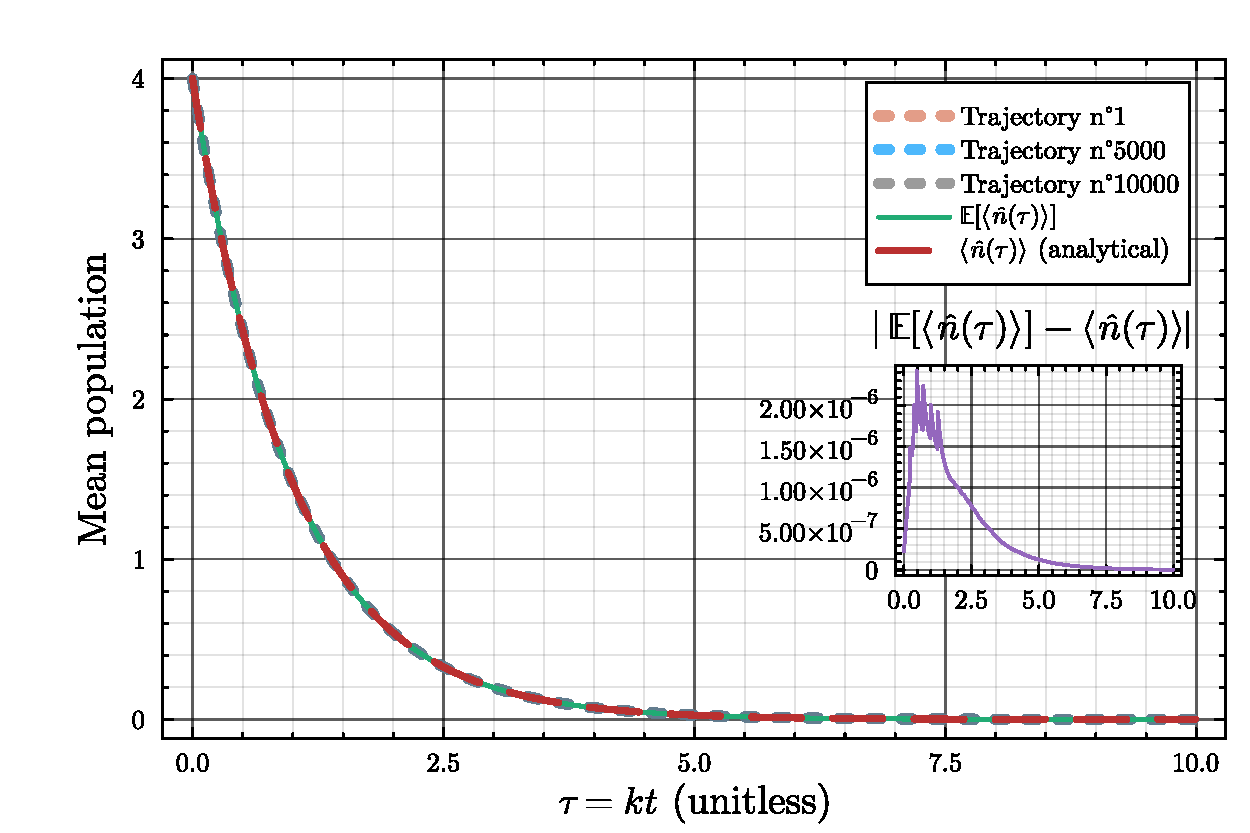
\includegraphics[width=\textwidth]{MCH/Pop_10000.pdf}
        \caption{The evolution of the mean population of the harmonic oscillator with respect to dimensionless time $\tau$ compared to the unconditional evolution of the mean population.}
        \label{fig:MCHpop}
    \end{subfigure}
    \\
    \begin{subfigure}[t]{0.58\textwidth}
        \centering
        
\includegraphics[width=\textwidth]{MCQ/histo.pdf}
        \caption{The histogram of simulation jump times $T$ of every simulations compared to the analytical Lindblad PDF.}
        \label{fig:MCHhist}
    \end{subfigure}
    
    \caption{Results obtained from the Monte Carlo simulation of a harmonic oscillator under continuous photo-detection of its environment. }
    \label{fig:MCHglobale}
\end{figure}o calculate $\expval{\hat{n}}{\psi_0(\tau)}$ after some steps. To do so, we might want to express this evolved state as a coherent state before any calculation. Indeed,
\begin{equation}
    \ket{\tilde{\psi}_0(t)} = e^{\gamma(t) a^\dagger a}\ket{\alpha_0},
\end{equation}
where we used $\gamma(t)=-(i\omega_0+\frac{k}{2})(t-t_0)$ as a shorthand notation. By virtue of Eq.~(\ref{eq:coherentfock}), this state can be expressed as
\begin{equation}
    \ket{\tilde{\psi}_0(t)} = e^{-\frac{\abs{\alpha_0}^2}{2}}\sum_{n=0}^{+\infty} \frac{\alpha_0^n}{\sqrt{n!}}e^{\gamma(t) a^\dagger a}\ket{n} = e^{-\frac{\abs{\alpha_0}^2}{2}}\sum_{n=0}^{+\infty} \frac{\qty(\alpha_0 e^{\gamma(t)})^n}{\sqrt{n!}}\ket{n}.
\end{equation}
To force the apparition of a coherent state in the last expression, we set
\begin{equation} 
    \alpha(t)=\alpha_0 e^{\gamma(t)}=\alpha_0 e^{-i\omega_0(t-t_0)}e^{-\frac{k}{2} (t-t_0)}. 
\end{equation}
Using the calculation trick of multiplying a term by its inverse, we eventually find
\begin{equation}
    \ket{\tilde{\psi}_0(t)} = e^{\frac{\abs{\alpha(t)}^2}{2}}e^{-\frac{\abs{\alpha(t)}^2}{2}}\ket{\tilde{\psi}_0(t)} = e^{-\frac{\abs{\alpha_0}-\abs{\alpha(t)}^2}{2}}\ket{\alpha(t)}.
\end{equation}
This state is easy to normalize since $\braket{\beta}=1$ for any coherent state $\ket{\beta}$. Therefore, we proved that starting with a coherent state $\ket{\alpha_0}$ assures that
\begin{equation}
    \ket{\psi_0(t)} = \ket{\alpha(t)} = \ket{\alpha_0 e^{-i\omega_0(t-t_0)}e^{-\frac{k}{2} (t-t_0)}}.
\end{equation}
The mean population can be simply evaluated thanks to $\expval{\hat{n}}{\beta} = \abs{\beta}^2$ for any coherent state $\ket{\beta}$. This relation implies that
\begin{equation}
    \expval{\hat{n}}{\psi_0(t)} = \abs{\alpha_0}^2 e^{-k(t-t_0)} \Leftrightarrow \expval{\hat{n}}{\psi_0(\tau)} = \abs{\alpha_0}^2 e^{-\tau},
\end{equation}
the right hand equation being simply the same as the left one with the dimensionless conversion $kt=\tau$ (along with the fact that $t_0=0$). If we now compare this result with the unconditional evolution in Eq.~(\ref{eq:uncondMCH}), we realize that they are exactly the same. This result explains why the errors between the average curve, the unconditional curve and the no-jump curve is so small. We seem to have find an initial system which is not bothered by the photo-detection measurement of its environment. Obviously, the system's population still jumps to different levels as the Figure~\ref{fig:MCHhist} shows, so their is still a tiny difference between the average conditional curve and the unconditional curve. 

\subsection{The qubit under homodyne detection of its environment}

For the homodyne measuring process we simulate the evolution of the conditional state with the function \verb|smesolve| from \verb|QuantumToolbox.jl|. The Hamiltonians and initial states are the same for each system but we chose to work with density matrices in the programs (here \verb|XHomodyneQubit.jl| and \verb|PHomodyneQubit.jl|) for demonstrative purpose. 

In the qubit case, one quickly realizes that the $0$ and $\pi/2$ quadratures are interesting operators to measure because they are linked to the correlation of the state. To show this, we need to work on the expression of $\expval{\sigma_\theta} = \mathrm{Tr}\qty[\rho(t)\sigma_\theta]$ with a general density matrix $\rho$, in which we define the qubit's quadrature operator by  
\begin{equation}
    \sigma_\theta = \frac{\sigma_- e^{-i\theta} + \sigma_+ e^{i\theta}}{\sqrt{2}}.
\end{equation}
This expression can be developed to let the correlations appear explicitly, yielding
\begin{equation}
    \expval{\sigma_\theta} = \frac{\rho_{eg} e^{-i\theta} + \rho_{ge} e^{i\theta}}{\sqrt{2}} = \abs{\rho_{eg}}\frac{e^{i(\varphi-\theta)}+e^{i(\theta-\varphi)}}{\sqrt{2}},
\end{equation}
where we used the exponential notation for the correlations (complex scalars). In particular, since $\rho_{ge}=\rho_{eg}^*$ we can write that $\rho_{eg}=\abs{\rho_{eg}}e^{i\varphi}$ and that $\rho_{ge}=\abs{\rho_{eg}}e^{-i\varphi}$. We can recognize the expression of a cosinus, hence
\begin{equation}
    \expval{\sigma_\theta} = \sqrt{2} \abs{\rho_{eg}} \mathrm{cos}\qty(\varphi-\theta).
\end{equation}
In particular, the aforementioned quadratures are therefore
\begin{equation}
    \expval{\sigma_0} = \sqrt{2} \abs{\rho_{eg}} \mathrm{cos}\qty(\varphi)=\sqrt{2}\mathrm{Re}\qty{\rho_{eg}}, \quad \expval{\sigma_{\pi/2}} = \sqrt{2} \abs{\rho_{eg}} \mathrm{sin}\qty(\varphi)=\sqrt{2}\mathrm{Im}\qty{\rho_{eg}}.
\end{equation}
The simulations yield the graphs in Figure~\ref{fig:HQglobale} where we can compare the averaged quadratures with the analytical unconditional quadratures. To find the expressions of these analytical curves, we used the OQS theory~\cite{Breuer}, which gives
\begin{equation}
    \rho_{eg}(t) = \rho_{eg}(0)e^{-\qty(\frac{k}{2}+i\omega_0)t}
\end{equation}

\begin{figure}[h]
    \centering
    \begin{subfigure}[t]{0.6\textwidth}
        \centering
        
\includegraphics[width=\textwidth]{HQ/Xquadrature.pdf}
        \caption{The evolution of $\sqrt{2}\mathrm{Re}\qty{\rho_{eg}}$ of the qubit with respect to dimensionless time $\tau$ compared to the unconditional evolution of the same quantity.}
        \label{fig:HQXquad}
    \end{subfigure}
    \\
    \begin{subfigure}[t]{0.6\textwidth}
        \centering
        
\includegraphics[width=\textwidth]{HQ/Pquadrature.pdf}
        \caption{The evolution of $\sqrt{2}\mathrm{Im}\qty{\rho_{eg}}$ of the qubit with respect to dimensionless time $\tau$ compared to the unconditional evolution of the same quantity.}
        \label{fig:HQPquad}
    \end{subfigure}
    
    \caption{The evolution of two qubit quadratures obtained by simulating continuous homodyne detection of the qubit's environment. }
    \label{fig:HQglobale}
\end{figure}

blablabla

\begin{figure}[h]
    \centering
    \begin{subfigure}[t]{0.6\textwidth}
        \centering
        
\includegraphics[width=\textwidth]{HQ/XquadSingleError.pdf}
        \caption{The evolution of $\sqrt{2}\mathrm{Re}\qty{\rho_{eg}}$ of the qubit with respect to dimensionless time $\tau$ compared to the unconditional evolution of the same quantity.}
        \label{fig:HQXquaderr}
    \end{subfigure}
    \\
    \begin{subfigure}[t]{0.6\textwidth}
        \centering
        
\includegraphics[width=\textwidth]{HQ/PquadSingleError.pdf}
        \caption{The evolution of $\sqrt{2}\mathrm{Im}\qty{\rho_{eg}}$ of the qubit with respect to dimensionless time $\tau$ compared to the unconditional evolution of the same quantity.}
        \label{fig:HQPquaderr}
    \end{subfigure}
    
    \caption{The evolution of two qubit quadratures obtained by simulating continuous homodyne detection of the qubit's environment. }
    \label{fig:HQerrglobale}
\end{figure}
\newpage

\section*{\Huge Conclusion}
This work, carried out in the framework of an internship during the final months of a Master's degree, has been dedicated to understanding and studying the evolution of quantum open systems under continuous measurement of their environment. We therefore described the fundamental theories of closed quantum systems up to the unconditional master equation describing the evolution of open quantum systems. In particular, the derivation of the Lindblad master equation presented in the first chapter was performed within the input-output formalism under the Born-Markov approximations. 

The heart of our study aimed on the impact of continuous monitoring of the environment of open quantum systems in the second chapter. This impact is specifically crystallized in the conditional trajectories depending on which process of measurement is made on the environment. We studied two of these processes in details, the first being described by a jump-like output signal (photo-detection), while the second one being characterized by a continuous diffusive signal (homodyne detection). The studied processes have been modeled with stochastic processes, namely a Poisson process and a Wiener process. We also extended this study to the theoretical expressions allowing to simulate trajectories, whose underlying stochastic differential equations (called stochastic master equations) are initially non-linear and challenging to solve. This has been made possible by deriving linear quantum trajectories and by deriving the Kraus operators formalism. Finally, we simulated some trajectories of a qubit and a harmonic oscillator under the continuous monitoring of their environment. These simulations clearly highlighted the validity of the theoretical results since the averaged trajectory is perfectly coincides with the unconditional trajectory (when the number of trajectories tends to infinity). This property explains precisely why the derivation of a specific stochastic master equation is called an ``unravelling'' of the Lindblad unconditional master equation.

Beyond the theoretical results established in this report, several directions can extend this work. While our study focused exclusively on a vacuum bath, a natural next step would be to incorporate thermal environments~\cite{W93}. Furthermore, introducing more realistic descriptions would bridge the gap toward experimental reality, such as accounting for imperfect measurement processes and detector inefficiencies~\cite{Albarelli}. In the same vein, the framework of homodyne detection can be generalized to the so-called ``heterodyne'' or even "general-dyne" detection schemes~\cite{Albarelli, Jacobs2006, Genoni14}. Beyond the standard systems considered here, the scientific community studied more complex system, e.g., a single nonlinear Kerr resonator whose Hamiltonian features quadratic driving terms~\cite{Bartolo2017}. Finally, the theory of continuous quantum measurement could be naturally integrated into the (huge) framework of quantum estimation and metrology~\cite{PARIS2009, Rossi2020}.
\newpage

\appendix
\setlength{\parskip}{2mm}\setlength{\parindent}{6mm}
\renewcommand{\thesubsection}{\thesection.\alph{subsection}\char41}
\numberwithin{equation}{section}
\renewcommand{\theequation}{\thechapter.~\arabic{equation}}
\chapter{Superposition of states VS statistical mixture}\label{ann:statmix}
In order to illustrate the concepts of superposition of states and statistical mixture, let us consider to observables $A,B$ such that
\begin{align*}
    \forall i\in\qty{1,2},\quad A\ket{\phi_i}&=a_i\ket{\phi_i},\\
    \forall i\in\qty{1,2},\quad B\ket{\psi_i}&=b_i\ket{\psi_i}.
\end{align*}
We can define a state $\ket{\Psi}$ in superposition of the eigenstates of the observable $B$:
\begin{equation}
    \boxed{\ket{\Psi} = \lambda_1\ket{\psi_1}+\lambda_2\ket{\psi_2}},
\end{equation}
where $\qty(\lambda_1,\lambda_2)\in\mathbb{C}^2$ such that $\abs{\lambda_1}^2+\abs{\lambda_2}^2=1$. We thus observe the result $b_i$ with following probability
\begin{equation}
    \forall i\in\qty{1,2},\quad\mathbb{P}_\Psi[b_i]=\abs{\braket{\psi_i}{\Psi}}^2=\abs{\lambda_i}^2\equiv p_i.
\end{equation}
If now we measure the system in order to find one of the eigenvalues of $A$, $a_1$ for example, we find
\begin{align}
    \mathbb{P}_\Psi[a_1] &= \abs{\braket{\phi_1}{\Psi}}^2\\
    &= \abs{\lambda_1\braket{\phi_1}{\psi_1}+\lambda_2\braket{\phi_1}{\psi_2}}^2\notag.
\end{align}
Moreover, by observing that $\forall i\in\qty{1,2},\quad\mathbb{P}_{\psi_i}[a_1]=\abs{\braket{\phi_1}{\psi_i}}^2$, we finally find that
\begin{equation}
    \boxed{\mathbb{P}_\Psi[a_1] = p_1\mathbb{P}_{\psi_1}[a_1]+p_2\mathbb{P}_{\psi_2}[a_1] + 2\Re{\lambda_1\lambda_2^*\braket{\phi_1}{\psi_1}\braket{\phi_1}{\psi_2}^*}}.
\end{equation}
We will now prepare a state with the same probabilities $\mathbb{P}[b_i]\equiv p_i$ but which is completely different.

A statistical mixture can be well understood by the following thought experiment:
\begin{itemize}
    \item We want to prepare $N$ states in total using the eigenstates $\qty{\psi_1,\psi_2}$ of $B$.
    \item We prepare $n_1$ states in $\ket{\psi_1}$.
    \item We prepare $n_2$ states in $\ket{\psi_2}$, so $n_1+n_2=N$.
\end{itemize}
At this point, we have a set of $N$ systems that we can use. However, if we pick a state randomly the probability to pick $\ket{\psi_i}$ depends on the fraction of it $p_i=\frac{n_i}{N}$. This fraction $p_i$ coincides theoretically with the previous probability $P_\Psi[b_i]$ for the superposition of states: it represents the probability to find the state $\ket{\psi_i}$ from the general state. If we now use the observable $A$ to measure the system we picked, the probability to find the result $a_1$ becomes
\begin{equation*}
    \mathbb{P}_\mathrm{sm}[a_1] = \frac{n_1\mathbb{P}_{\psi_1}[a_1]+n_2\mathbb{P}_{\psi_2}[a_1]}{N} = p_1\mathbb{P}_{\psi_1}[a_1]+p_2\mathbb{P}_{\psi_2}[a_1],
\end{equation*}
by using the law of total probability. Therefore,
\begin{equation}
    \boxed{\mathbb{P}_\mathrm{sm}[a_1] =p_1\mathbb{P}_{\psi_1}[a_1]+p_2\mathbb{P}_{\psi_2}[a_1]}.
\end{equation}
By comparing the last two boxed equations, one can realize that the mathematical expression for the same probability is written differently depending on if we use a superposition of states or a statistical mixture. However, the probability of the statistical mixture is present in the expression of probability of the superposition of states. This difference of formula for the same probability therefore proves that the Dirac formalism $\ket{\psi}$ cannot represent the kind of system whose probability comes from a statistical mixture. It is in fact impossible to represent a statistical mixture with a pure state. Instead, we need to use the density matrix 
\begin{equation}
    \rho_\mathrm{sm} = p_1\ketbra{\psi_1}+p_2\ketbra{\psi_2},
\end{equation} 
so that,
\begin{equation}
    \mathbb{P}_{\rho_\mathrm{sm}}[a_1] = p_1\mathbb{P}_{\psi_1}[a_1]+p_2\mathbb{P}_{\psi_2}[a_1],
\end{equation}
because by definition $\mathbb{P}_{\rho_\mathrm{sm}}[a_1]=\Tr{\rho_\mathrm{sm}\ketbra{\phi_1}}$.

\newpage
\chapter{Representations of quantum mechanics}\label{ann:pictures}
\section*{Brief complement of quantum mechanics}
An average is defined in quantum mechanics by
\begin{align*}
    \expval{O}_\psi&=\expval{O}{\psi},\\
    \expval{O}_\rho&=\Tr{\rho O},
\end{align*}
where the subscripts $\ket{\psi}$ and $\rho$ refer respectively to the representation of pure states or
to density matrix more general formalism. 
\section{Schrödinger and Heisenberg pictures}\noindent
In the Schrödinger picture we saw that $\ket{\psi(t)}=U(t)\ket{\psi}$, where $U(t)=e^{-\frac{i}{\hbar}Ht}$ in the case of a time-independent Hamiltonian with $t_0=0$. Nevertheless, the following results can be derived in the general case of a time dependent Hamiltonian,~\cite{Breuer}. Considering the average value of an observable $A_S(t)$ in the Schrödinger picture (in this picture, the time-dependence of an observable can only be explicit), we find
\begin{align}
    \expval{A(t)} &= \expval{A_S(t)}{\psi(t)}\nonumber\\
    &= \expval{U^\dagger(t,t_0)A_S(t)U(t,t_0)}{\psi(t_0)}\\
    &= \expval{A_H(t)}{\psi}_H.
\end{align}
This calculation naturally reveals the Heisenberg representation of observables and states. Indeed, we have that $\ket{\psi(t_0)}_S\equiv\ket{\psi}_H$ which links both pictures at the initial time $t_0$. Furthermore, we can link both representation at all time by calculating the evolution of an observable in the Heisenberg picture:
\begin{equation}
    \boxed{\dert{A_H} = \frac{i}{\hbar}\left[H_{H},A_{H}\right] + \derpart{A_S}\label{eq:HSlink}}.
\end{equation}
This equation leads to the famous \textit{Ehrenfest theorem} analogous in quantum mechanics:
\begin{equation}
    \boxed{\dert{\expval{A}}=\frac{i}{\hbar}\expval{\qty[H(t),A(t)]}+\expval{\derpart{A}}}.
\end{equation}
We observe that if the observable doesn't depend explicitly on time, then the dynamics of the operator is fully described in the Heisenberg picture.

\section{Interaction picture}\noindent
As mentioned in the Section~\ref{OQS}, we can represent the coupling between $S$ and $E$ with an interaction Hamiltonian such that
\begin{align}
    H_T = \overbrace{H_S\otimes\mathbb{I}_E+\mathbb{I}_S\otimes H_E}^{H_0}+H_I.
\end{align}
Knowing that $\ket{\psi(t)}_S=U(t,t_0)\ket{\psi}_S$, we can write that
\begin{equation}\label{eq:evolrhoU}
    \rho_S(t) = U(t,t_0)\rho_{S}(t_0)U^\dagger(t,t_0).
\end{equation}
The evolution operator $U$ is the solution of the Schrödinger equation for the total system $T$. We know that the free system (dynamically governed by $H_0$) also follows unitary dynamics, which is described by $U_0$. Thus, we can define the interaction unitary operator $U_I$ as
\begin{align}
    U_I(t,t_0) &= U_0^\dagger(t,t_0)U(t,t_0)\\
    \Leftrightarrow U(t,t_0) &= U_0(t,t_0)U_I(t,t_0)\label{eq:Utotal}
\end{align}
If we now try to calculate the average of an operator (in the total space $\mathcal{H}_T$) using the Schrödinger picture, we can find a new interesting relation by injecting the Eq.~(\ref{eq:Utotal}) in the Eq.~(\ref{eq:evolrhoU}) and then into the following average:
\begin{align*}
    \expval{O(t)} &= \Tr{\rho_{S}(t)O_S(t)}\\
    &= \mathrm{Tr}\,[\underbrace{U_I(t,t_0)\rho_{S}(t_0)U_I^\dagger(t,t_0)}_{\tilde{\rho}(t)}\,\underbrace{U_0^\dagger(t,t_0)O_S(t)U_0(t,t_0)}_{\tilde{O}(t)}].
\end{align*}
We can thus define in the interaction picture:
\begin{align}
    \tilde{\rho}(t)&=U_I(t,t_0)\rho_{S}(t_0)U_I^\dagger(t,t_0),\label{eq:rhoIS}\\
    \tilde{O}(t) &= U_0^\dagger(t,t_0)O_S(t)U_0(t,t_0)\label{eq:obsIS}.
\end{align}
We can now reverse the Eq.~(\ref{eq:evolrhoU}) and then use the Eq.~(\ref{eq:Utotal}) to get
\begin{equation*}
    \rho_S(t_0) = U^\dagger(t,t_0)\rho_S(t)U(t,t_0) = U_I^\dagger(t,t_0)U^\dagger_0(t,t_0)\rho_S(t)U_0(t,t_0)U_I(t,t_0),
\end{equation*}
and, by injecting this into the Eq.~(\ref{eq:rhoIS}), we get
\begin{equation}
    \tilde{\rho}(t) = U^\dagger_0(t,t_0)\rho_S(t)U_0(t,t_0).
\end{equation}
This result is obvious because a density matrix is also an operator and thus respects the Eq.~(\ref{eq:obsIS}).
In the end, we find the results used in the main part of this document:
\begin{equation}
    \boxed{\tilde{\rho}(t)=U_I(t,t_0)\rho_{S}(t_0)U_I^\dagger(t,t_0)= U^\dagger_0(t,t_0)\rho_S(t)U_0(t,t_0)}.
\end{equation}
By working on the Liouville-von Neumann equation, one can show that by jumping into the interaction picture the dynamics do not depend anymore on the free Hamiltonian $H_0$:
\begin{equation}
    \qty(\dert{\rho}=-\frac{i}{\hbar}\qty[H_T,\rho])\Leftrightarrow\qty(\dert{\tilde{\rho}}=-\frac{i}{\hbar}\qty[\tilde{H}_I,\tilde{\rho}]),
\end{equation}
where $\tilde{H}_I=U_0^\dagger(t,t_0)H_I U_0(t,t_0)$ as defined. It is thus usual to work in this representation to get rid of free dynamics terms, and then jump back to the Schrödinger picture to recover the proper dynamics of the system.
\subsubsection{Further discussion}\noindent
As seen in Eq.~(\ref{eq:rhoIS}), a state evolves in the interaction picture with a relation depending on $U_I$, which has been defined as $U_I=U_0^\dagger U$. It is possible to show from this definition that $U_I$ is subject to the following differential equation
\begin{equation}
    \dert{U_I}=-\frac{i}{\hbar}\tilde{H}_I U_I,
\end{equation}
where we recall that $\tilde{H}_I=U_0^\dagger H_I U_0$ by definition of the interaction picture. If we now consider the evolution  
\newpage
\chapter{Simple stochastic differential equations}\label{ann:stieltjes}
We want here to justify the expression of Eq.~(\ref{eq:SMEphotodet}) where we discarded terms proportional to $\mathrm{d}N_t \dt$. We recall that $\mathrm{d}N_t$ is a Poisson increment, meaning that $\mathrm{d}N_t^2 = \mathrm{d}N_t$. Moreover, we work in a case where the only values this increment can have is 0 or 1, with probability $\mathbb{P}\qty[\mathrm{d}N_t=0] = 1-\lambda_t \dt\approx 1$ and $\mathbb{P}\qty[\mathrm{d}N_t=1] = \lambda_t \dt\approx 0$.

When dealing with stochastic master equation, it is useful to integrate them in order to understand the underlying mathematical background. Note that the real interest of the SME is to integrate it in order to find the expression of a state. We consider the case of a stochastic differential equation, such as
\begin{equation}
    \mathrm{d}f = a~\dt + b~\mathrm{d}N_t + c~\mathrm{d}N_t\dt,
\end{equation}
where $a,b,c\in\mathbb{R}$, they could be functions of time but we prefer to simplify the discussion. We are going to integrate this equation from $t_0$ to $T$, to do so we discretize the time as $t_0<t_1<\cdots<t_n=T$. We thus express the $i$-th time as $t_i = t_0+i\delta t$, in particular when $i=n$: $T=t_0+n\delta t \Leftrightarrow n = \frac{T-t_0}{\delta t}$. This shows that when $n\rightarrow +\infty$, we automatically have $\delta t\rightarrow 0^+$. This discretization allows us to define the first integral with measure $\dt$ as
\begin{equation}
    \int_{t_0}^T a~\dt = a \lim_{n\rightarrow +\infty} \sum_{i=0}^{n-1} (t_{i+1}-t_i) = a \lim_{n\rightarrow +\infty} (t_n-t_0) = a (T-t_0),
\end{equation}
which is simply a Riemann integral. The reason we find a finite quantity is hidden in the fact that we sum infinitely $\delta t$ while $\delta t$ is going to 0 at the same time. If we now consider the second integral, that we understand as a Stieltjes integral, we obtain
\begin{equation}
    \int_{t_0}^T b~\mathrm{d}N_t = b \lim_{n\rightarrow +\infty} \sum_{i=0}^{n-1}\qty[N(t_{i+1},t_0)-N(t_i,t_0)] = b \sum_{j=0}^{k-1} 1 = bk,
\end{equation}
where $N(t_{i+1},t_0)-N(t_i,t_0)=0$ most of the time and $1$ only $k$ times, according to the probability law followed by the Poisson increment. This result, when applied to the third integral, gives 
\begin{equation}
    \int_{t_0}^T c~\mathrm{d}N_t\dt = c \sum_{j=0}^{k-1}\dt=c k \dt\approx 0,
\end{equation}
in the Stieltjes definition of the integral, which explains why we can neglect $\mathrm{d}N_t\dt$ in the photo-detection SME.
\newpage
\chapter{Homodyne detection in quantum optics}\label{app:homodyne}
As explained in Section~\ref{sec:homodyne}, the homodyne detection creates a continuous signal containing information on the quadrature of the physical system of interest. We use the notations of Figure~\ref{fig:homodyne}, i.e., the system field is labelled by the system annihilation operator $\hat{a}$ (and is now an input of the homodyne detection process). We also use another input signal which is a coherent field labelled by its annihilation operator $\hat{b}$. Moreover, we use a 50:50 beam-splitter to form two output fields labelled $\hat{c}$ and $\hat{d}$ which are then measured by two photo-detectors, as depicted in the aforementioned figure. The quadrature of the system is defined by
\begin{equation}
    \hat{a}_\theta=\frac{\hat{a}^\dagger e^{i\theta}+\hat{a}e^{-i\theta}}{\sqrt{2}}.
\end{equation}

Quantum optics~\cite{Gerry2023} assures that, after the beam-splitter, the output fields are 
\begin{equation}
    \hat{c}=\frac{\hat{a}+i\hat{b}}{\sqrt{2}},\qquad
    \hat{d}=\frac{\hat{b}+i\hat{a}}{\sqrt{2}}.
\end{equation}
These relations hold when the beam-splitter is 50:50. Hence, this exact process is called ``balanced'' homodyne detection. We explained in Section~\ref{sec:photodet} that the photo-detector signal is proportional to the mean value of the occupation number. Thus, $I_c \propto \expval{\hat{c}^\dagger \hat{c}}$ and $I_d \propto \expval{\hat{d}^\dagger \hat{d}}$. Therefore, the difference of photo-currents is
\begin{equation}\label{eq:D2}
    I_d-I_c \propto i\expval{\hat{a}^\dagger\otimes\hat{b}-\hat{a}\otimes\hat{b}^\dagger}.
\end{equation}
As explained, the field input labelled by $\hat{b}$ is a coherent field. We denote this field as $\ket{\beta}$ so that $\hat{b}\ket{\beta}=\beta\ket{\beta}$, where $\beta=\abs{\beta}e^{i\phi}\in\mathbb{C}$. If we denote the input state of the system as $\ket{\psi}$, then the total input state is $\ket{\psi_\text{in}}=\ket{\psi} \otimes \ket{\beta}$. We can therefore explicit the average in Eq.~(\ref{eq:D2}) as
\begin{equation}
    I_d-I_c \propto i\abs{\beta}\expval{(\hat{a}^\dagger e^{i\phi}-\hat{a}e^{-i\phi})}{\psi} = \abs{\beta}\expval{(\hat{a}^\dagger e^{i\theta}+\hat{a}e^{-i\theta})}{\psi},
\end{equation}
where we introduced $\theta=\phi-\pi$. Therefore, we have briefly shown that homodyne detection signal is proportional to the quadrature of the system $\hat{a}_\theta$.

\printbibliography%
\end{document}